\documentclass[10pt,a4paper]{article}
\usepackage[utf8]{inputenc}
\usepackage[english]{babel}
\usepackage{graphicx}
\usepackage{lmodern}
\usepackage{kpfonts}
\usepackage{subcaption}
\usepackage{dsfont}
\usepackage{wrapfig}
\usepackage[left=2cm,right=2cm,top=2cm,bottom=2cm]{geometry}
\usepackage{hyperref}
\usepackage{xcolor}
\usepackage{enumitem}
\usepackage{wrapfig}
\title{Kahn}
\author{Megi Dervishi, Nizar Ghandri, Christophe Saad}
\date{\today}

\begin{document}


\maketitle
\section{Introduction}
There are three main implementations of Khan that we have achieved: Sequential, Pipes and Network. For the network there are two sub-implementations: one running in one machine (section 1.1) referred in the rest of the report as just Network and one running in two machines (section 1.2) referred in the report as Network2window. There are also the applications: Mandelbrot, Tictactoe, K-means and Example.ml. These applications should run normally no matter if the kahn implementation is Sequential, Pipes or Network. However when the kahn implementation is Network2window then the applications which are able to work with it are only Tictactoe2window and Example.ml. Hence why we have two sub-implementations of the Network. We shall explain the reason behind it in the following section. The github repository for the project is \href{https://github.com/xopheS/kpn}{\color{blue}Github}.

\section{Khan implementations }

\subsection{Network}
This implementation of Khan aims at running the Kahn processes in parallel on a machine and making them communicate through sockets. It makes use of the module \texttt{Unix} for creating a classic TCP socket communication with an IPv4 or IPv6 address; makes use of the module \texttt{Marshal} to convert the value into bytes in order to be sent/received in the channel. The \texttt{put( value, output)} function makes use of the unix function \texttt{Unix.send} to send the particular value through the socket \texttt{output} and the \texttt{get(input)} function makes use of \texttt{Unix.receiv} to receive a particular value. The \texttt{doco} function takes a list of processes and runs them in parallel through the \texttt{Thread} module. The most important function is probably the \texttt{new\_channel} function. The Network implementation relies on the fact that all the Kahn processes communicating are ran in parallel on the same machine. Hence it suffices to create 'circular' channels from the local machine to itself and then distribute the \texttt{in\_channel} and \texttt{out\_channel} within the local processes. This is the structure followed in Example.ml, Mandelbrot.ml, Tictactoe.ml.   We summarize the typical behavior of the khan network with sockets in one machine in the following diagram:
\begin{figure}[h!]
   \centering
   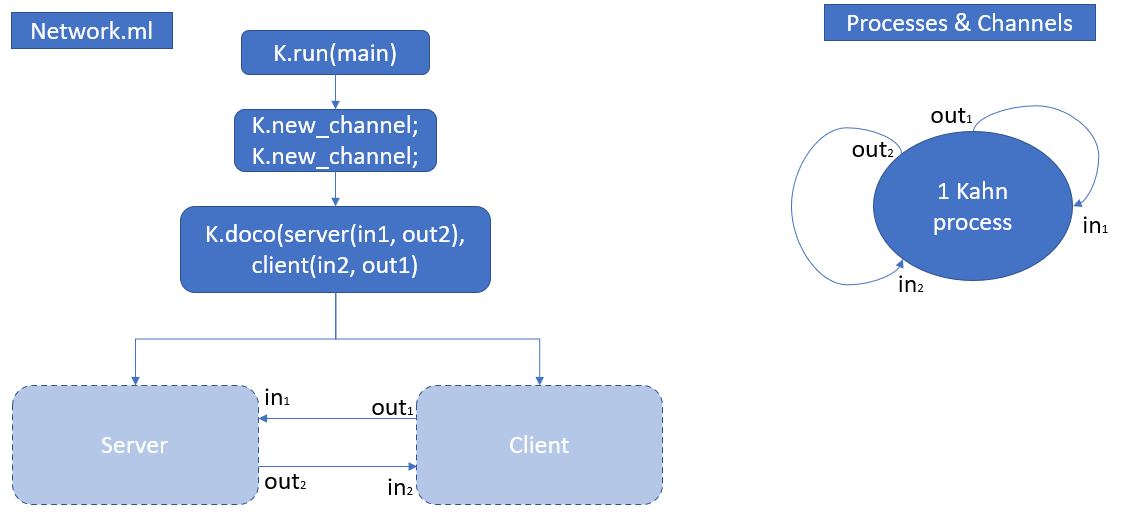
\includegraphics[width = 0.75\textwidth]{diagram1.png}
   \caption{Diagram of the functioning of the communications for the Network implementation.}
   \label{fig:my_label}
\end{figure}

\subsection{Network2Window}
This implementation of Khan aims at being able to connect Kahn processes which run on separate machines. The fundamental difference with the Network implementation resides in the \text{new\_channel} function. This is due to the fact that now channels connect two separate machines and hence two distinct Kahn processes (A, B) that cannot communicate with each other through any other means. This means that it is impossible for one \texttt{K.new\_channel} function to create a channel. This is because if A wants to create a channel with B then A must open two of his sockets wait for B to connect, accept the connection of B, connect in return to B and finally B must accept A's connection. This is resumed in the diagram below.

\begin{figure}[h!]
   \centering
   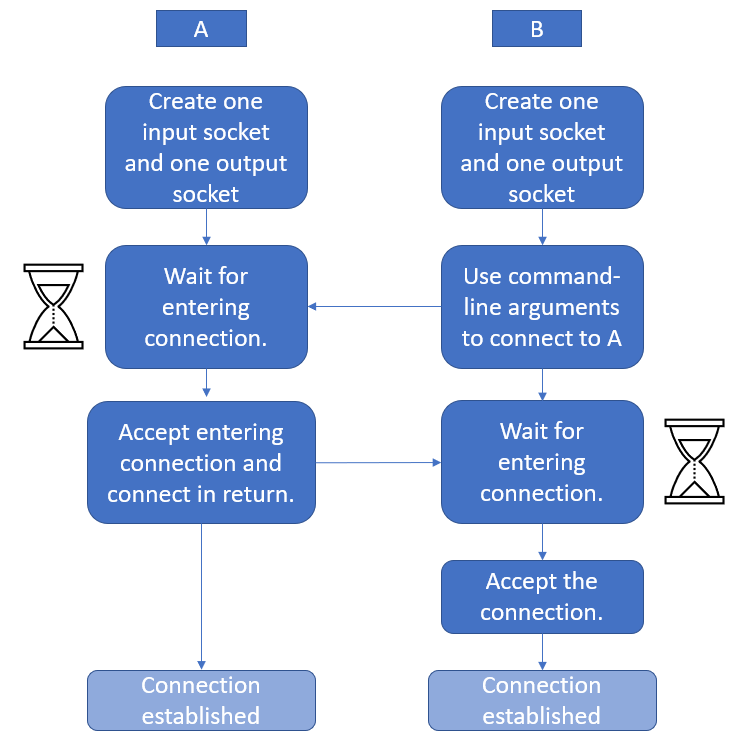
\includegraphics[width = 0.5\textwidth]{diagram3.png}
   \caption{Diagram of the functioning of the channel creation for Network2Window.}
   \label{fig:my_label}
\end{figure}

As we can see the algorithm for channel creation on machine A is different than the one on machine B. We hence have two options. The first is that both machines run \texttt{K.new\_channel} but one of them sets a flag like \texttt{K.is\_A} which \texttt{K.new\_channel} recognizes in order to switch behavior accordingly. The second is to add a new separate function like \texttt{connect\_by\_name} which corresponds to the algorithm of B while A runs \texttt{new\_channel}. For the purpose of clarity and simplicity we opted for the second option. This also means that the Network2Window implementation will not be able to run the other example programs without some minor adjustments as is done in \texttt{Example.ml}. To explicit this we show how the behavior in figure 1 is modified when using Network2Window in figure 3.

\begin{figure}[h!]
   \centering
   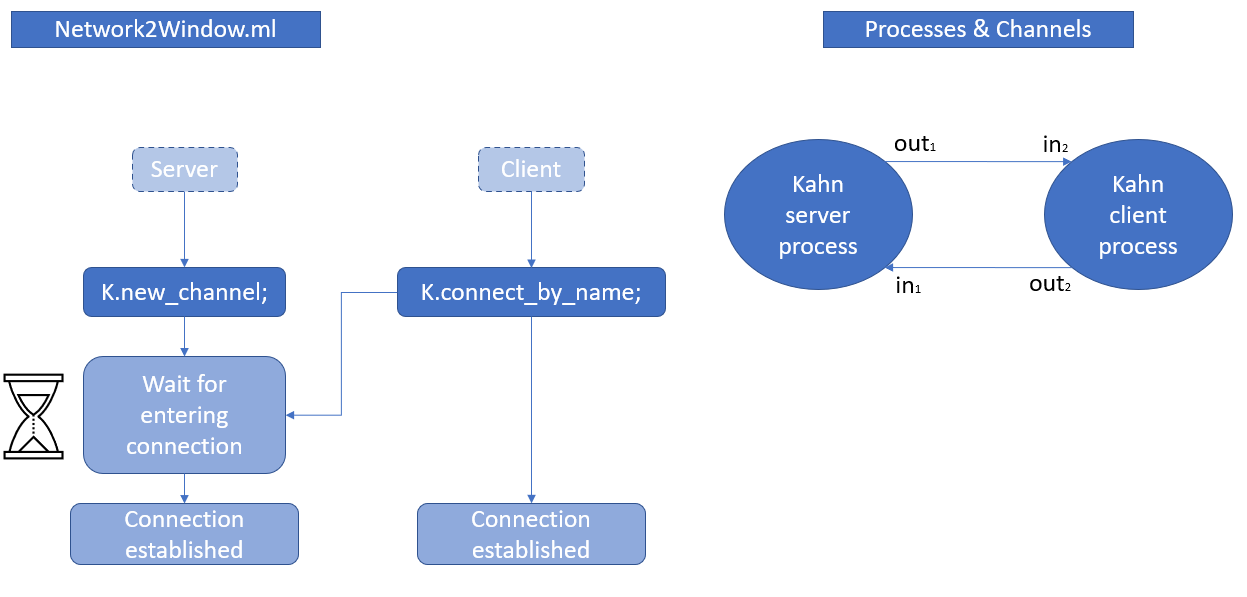
\includegraphics[width = 0.75\textwidth]{diagram2.png}
   \caption{Diagram of the functioning of the communications for the Network2Window implementation.}
   \label{fig:my_label}
\end{figure}

\subsection{Sequential}
The implentation of the sequencial part is manly taken from the paper A poor man’s concurrency monad. We consider the process as a monad transformer which takes an action (which contains the actual computation) and link it a continuation. Its type is: $\quad \quad \texttt{type 'a process = ('a -> action) -> action}$.
\\The type action is $$\texttt{type action = Atom of (unit -> action) | Fork of action * action | Stop}$$
We use \texttt{Fork} to instanciate new processes and \texttt{Atom} to represent a computation.\\
In the \texttt{run} function, we recreate a pipeline containing the first \texttt{Fork} action to execute. Each time a \texttt{Fork} is executed, we push the two actions in the pipeline. When an \texttt{Atom} is read, we execute its computation and store his continuation back in the pipeline. This procedures ends when all the continuations are \texttt{Stop}.

\subsection{Pipes}

The implentation of the Unix processes part is mainly based on the POSIX interface. Its type is $$\texttt{type 'a process = unit -> 'a}$$
Computation is mostly based on the generation of heavy Unix processes through the $\texttt{fork}$ method from the Unix library.
Communication channel is an unnamed pipe, which is a file accessed through its channel in/out which are Unix file descriptors. Sending and receiving data (put and get functions) use the module \texttt{Marshal} to convert the value into bytes in order to be sent/received in the channel, and mostly rely on the Unix functions (write, read).

\section{Applications}
As we have previously mentioned there are 4 applications: Mandelbrot, Tictactoe, Tictactoe2window and K\_means. We briefly explain some of their main features and how to run them.
\subsection{Mandelbrot}
This application consits of the computation and visualization of the Mandelbrot set using the implemented kahn network.
The Mandelbrot set $\mathcal{M}$ is the set of complex numbers $c$ such that the point $z = 0$ of the polynomial $P_c(z) = z^2 + c$ has an orbit which remains bounded. \\
In other words, this set can be seen as the set of complex numbers $c$ for which the application $z_{n+1} = z_n + c$ starting from $0$ for $n \rightarrow \infty$ remains bounded.

\subsubsection{Properties}
A very useful property of the mandelbrot set which will make its computation easier is the following:
$$c \in \mathcal{M} \quad \Longleftrightarrow \quad |\mathcal{P}^n_c(0)| \leq 2 \quad \forall n\geq 0$$
The sequence is certainly divergent if the modulus of z crosses 2.

\subsubsection{Objective of Implementation}
Our objective is to compute and plot the Mandelbrot set $\mathcal{M}$ on a given window and range of complex numbers. 

\subsubsection{Evaluation of points}
We map each pixel of the graph to a complex value depending on a given origin and a zoom scale (radius around the origin).\\
A common method for evaluating a point and checking whether it belongs to $\mathcal{M}$ consists of iterating over the sequence described above starting from $0$. The algorithm stops when the maximum number of steps (given as input) is reached or if we find that $|z| > 2$ (from previous property). An obvious optimization technique would be testing $|z|^2 > 4$ in order to avoid the squared root operation of the modulus.

\subsubsection{Colors}
A naive implementation would be to use two colors, one for pixels which belongs to $\mathcal{M}$ and another for those that don't. Another implementation technique to visualize similarity in points would be to use the number of iterations needed for the evaluation loop to exit. We can then visualize the deep points (those which needed the maximum number of steps) and the border points.\\
In our algorithm, we use a technique to visualize the equipotential lines of $\mathcal{M}$.\\
We replace the threshold $2$ by another value $r$ which can be seen as the escape radius. We use as inputs $r$ and the number of iterations $n$ to compute the potential $$V(c) = \frac{\log (\max (1, |z_n|))}{2^n}$$
This technique stays coherent in the sense that $V(c) = 0$ if and only if $c \in \mathcal{M}$. More information about the potential and required adjustments \href{https://www.math.univ-toulouse.fr/~cheritat/wiki-draw/index.php/Mandelbrot_set#The_potential}{\color{blue}here}.


\subsubsection{Kahn processes}
We divide the output window into sections, each one will be handled by a process. We use one last process for plotting the resulting values of the processes computations.\\
Computing processes send points values (coordinates and color assigned) to the channel where they wait to be retrieved by the plotting process.

\subsubsection{Running mandelbrot}
The mandelbrot application can be ran with arguments (\texttt{arg default type})
\begin{itemize}[label={}]
\item \texttt{-w 1300 int} Width of the window
\item \texttt{-h 1000 int} Height of the window
\item \texttt{-n 1000 int} Number of iterations
\item \texttt{-p 1 int} Number of processes for computation (must divide width)
\item \texttt{-xo -0.5 float} Real part of origin
\item \texttt{-yo 0. float} Imaginary part of origin
\item \texttt{-z 1. float} Zoom value (radius around origin)
\item \texttt{-r 4. float} Escape radius value

\end{itemize}

\subsubsection{Some views}
\begin{itemize}[label={}]
\item \texttt{-xo -0.7463 -yo 0.1102 -z 0.005}
\item \texttt{-xo -0.7453 -yo 0.1127 -z 0.00065}
\item \texttt{-xo -0.16 -yo 1.0405 -z 0.026}
\item \texttt{-xo -0.925 -yo 0.266 -z 0.032}
\item \texttt{-xo -0.748 -yo 0.1 -z 0.0014}
\item \texttt{-xo -0.722 -yo 0.246 -z 0.019}
\item \texttt{-xo -0.235125 -yo 0.827215 -z 0.00004}
\item \texttt{-xo -0.81153120295763 -yo 0.20142958206181 -z 0.0003}
\end{itemize}


\subsection{Tictactoe}

This application aims at creating a classic Tic Tac Toe game between two players. As we have noted previously there were two versions of this game \texttt{tictactoe.ml} which works in one machine with the Sequential, Pipes and Network implementation and \texttt{tictactoe2window.ml} which works for the Network2Window implementation of Kahn. Apart from few details (which we shall explain)  \texttt{tictactoe2window.ml} and \texttt{tictactoe.ml} have essentially the same design structure.

\subsubsection{Design of the communication }

In a classic client/server architecture, the server would have to decide the execution and communication of the khan processes between the two clients. However with this implementation the server becomes a bottleneck. In our implementation the communication happens directly between the clients where one of them becomes the host.

\subsubsection{Structure of messages}
The messages that are sent through the channel fall into four categories (\texttt{MYM}, \texttt{FYI}, \texttt{STS}, \texttt{ERR}). When a message string is composed the first three letters of it are one of the above. Hence the receiving party can recognize the type of message being sent and act accordingly :
\begin{itemize}
\item \texttt{MYM} (Make your move) - messages the client-host asks the client to make their move
\item \texttt{FYI} (For your information) - usually send the tic tac toe board
\item \texttt{STS} (Status) - send the stage/status of the game i.e \texttt{Win of player}, \texttt{Draw}, \texttt{Continue}
\item \texttt{ERR} (Error) - There is an invalid move happening.
\end{itemize}
As mentioned above the \texttt{FYI} send the tic tac toe board which is an \texttt{Array} of size 9.
\subsubsection{Client (host)}
The client host (server as referred in the code) does most of the computation of the game. The "server" recursively does the following in the \texttt{server\_main}
\begin{enumerate}
\item Waits for himself to make a valid move (a move inside the board that was not previously filled).
\item Updates the board with the current move
\item Checks if there is a winner or draw; If yes then it sends the status to the client and game ends i.e. stops the connection.
\item Otherwise sends the board to the client and waits for a response.
\item When the client sends a move the host checks if the move is valid. If not then repeat step 4.
\item Otherwise repeat step 2 and 3. If game has not ended then go back to step 1.
\end{enumerate}
\subsubsection{Client }
The client has a simplier process. It only receives messages from the host and acts accordingly to the type of message received:
\begin{enumerate}
\item \texttt{MYM} makes a move by clicking on the board; the move is converted into an index of the array and then sent to the host.
\item \texttt{FYI} gets the board and displays it
\item \texttt{ERR} the client made a wrong move
\item \texttt{STS} receives the status of the game.
\end{enumerate}
All the following can be found in the \texttt{client\_main} function.
\subsubsection{Run}
To play the game Tic Tac Toe using the Network, Sequential or Pipes implementations run:\\\\
\text{\texttt{make tictactoe}}\\
\text{\texttt{./tictactoe.native}}\\\\
To play the game Tic Tac Toe using the Network2Window implementation run:\\\\
\text{\texttt{make tictactoe2}}\\
\text{\texttt{./tictactoe2window.native}} \quad and \quad \text{\texttt{./tictactoe2window.native -client -ipaddr [hostip]}}\\\\
Upon execution there is a graphic window appearing. The default measurements for the window are 1000 by 620 and the board is 600 by 600. The players could insert a move by simply clicking the position they like. The first player to play is \texttt{X} and the second \texttt{O}. If you want to customize the measurements of the window or port in which you play you could add the following arguments:\\\\
\texttt{-port x -length\_window x -width\_window x -length x -width x}
\subsection{K means}

"k-means clustering is a method of vector quantization, originally from signal processing, that aims to partition n observations into k clusters in which each observation belongs to the cluster with the nearest mean (cluster centers or cluster centroid), serving as a prototype of the cluster."
-Wikipedia

K-means is an example of a bulk synchronous parallel algorithm (BSP). BSP algorithms are composed from a sequence of supersteps, each of which contains:
\begin{itemize}
\item parallel computation, in which processes independently perform local computations and produce some values
\item communication, in which processes exchange data
\item barrier synchronisation, during which processes wait until every process finishes

\end{itemize}


Data-parallel programming models are typically a good fit for BSP algorithms, as each bulk synchronous phase can correspond to some number of data-parallel operations.


The whole implementation thus relies on the implementation of a \texttt{split\_workload} function that divides the data structure (Array) into equal parts. The number of parts is usually equal to the maximum number of processes that can be used.
Then every worker performs the computations (Array.map) on every part.
This would give us a \texttt{parallel\_map} that can only use up \texttt{number\_of\_processes} processes.
From there we use the \texttt{parallel\_map} with a fold left to code a parallel group by function.
Using these functions we code the K\_means module representing the core K means algorithm.
We also then add another module to run the K means algorithm on the Iris data set.
We use the Str library and their regex expressions to parse comma separated values files and import the data set.
Finally, we add two graphical components to the algorithm launcher:
\begin{itemize}
\item \texttt{plot.py}: A python module that plots the accuracy of the K means on the test and training data: the accuracy here is measure by the purity of the clusters.

\item \texttt{show\_points}: A use of the Graphics module in ocaml to plot the points the clusters and the means depending on any two features selected in the variables x\_axis and y\_axis.
\end{itemize}


\subsubsection{Usage}

Running the algorithm requires only one argument which is the number of processes used: $$\texttt{make k\_means}$$ $$\texttt{./k\_means.native 8}$$
It will run automatically on the Iris data set.

\end{document}